\documentclass[a4paper,10pt]{article}
\usepackage[utf8]{inputenc}
\usepackage[T1]{fontenc}
\usepackage[polish]{babel}
\usepackage{graphicx}
\usepackage{mathtools}

%opening
\title{Badanie złożoności obliczeniowej dwóch implementacji stosu}
\author{Szymon Leśniak}

\begin{document}

\maketitle

\section{Opis badania}

\par Dokonano implementacji stosu na liczby całkowite typu \verb+int+ 
za pomocą tablicy. Implementacji dokonano w dwóch wariantach: w każdym
z nich wielkość stosu nie była stała; przy próbie położenia liczby na
pełny stos dokonywano realokacji tablicy.

\par Przy zastosowaniu strategii inkrementacyjnej nowoalokowany stos miał
rozmiar o jeden większy niż dotychczas. Innymi słowy, stosowi zmieniano 
wielkość przy każdym położeniu nowego elementu. Analogicznie stos był
zmniejszany za każdym razem, gdy z niego zabierano liczbę.

\par Strategia podwajania miała na celu zmniejszenie częstotliwości realokacji
stosu. W tym celu rozmiar przy każdym przepełnieniu stosu jego rozmiar jest
powiększany dwukrotnie. Pamięć zajmowana przez stos była zwalniana wtedy, gdy
zapełnienie stosu spadło poniżej \(\frac{1}{4}\) zarezerwowanej dla niego pamięci.

\par Zbadany został czas napełnienia stosu dla różnych wielkości problemu. 
Dla każdej z wielkości badanie było powtórzone wielokrotnie. Implementacji 
dokonano w języku C++, przy użyciu systemu operacyjnego Ubuntu 13.10 oraz 
kompilatora g++ 4.8.1.

\section{Wyniki badania}

\par Wyniki są przedstawione w poniższych tabelach oraz na wykresie (skala 
log-log) 

\begin{center}
\begin{table}[h]
\caption{Wyniki badania strategii inkrementacyjnej}
\begin{tabular}{lll}
\textbf{Ilość liczb} & \textbf{Ilość badań} & \textbf{Średni czas [s]}\\
10 & 100 & 1,74\(\cdot 10^{-5}\)\\
100 & 75 & 0,000104885\\
1000 & 50 & 0,00203451\\
5000 & 25 & 0,0444254\\
10000 & 10 & 0,178434\\
100000 & 2 & 21,1769
\end{tabular}
\end{table}
\end{center}

\begin{center}
\begin{table}[h]
\caption{Wyniki badania strategii podwajania}
\begin{tabular}{lll}
\textbf{Ilość liczb} & \textbf{Ilość badań} & \textbf{Średni czas [s]}\\
10 & 100 & 1,79\(\cdot 10^{-5}\)\\
100 & 100 & 3,83\(\cdot 10^{-5}\)\\
1000 & 50 & 0,000271155\\
5000 & 50 & 0,000732078\\
10000 & 25 & 0,00115531\\
100000 & 15 & 0,0115602\\
1000000 & 5 & 0,114574
\end{tabular}
\end{table}
\end{center}

\begin{figure}[h]
 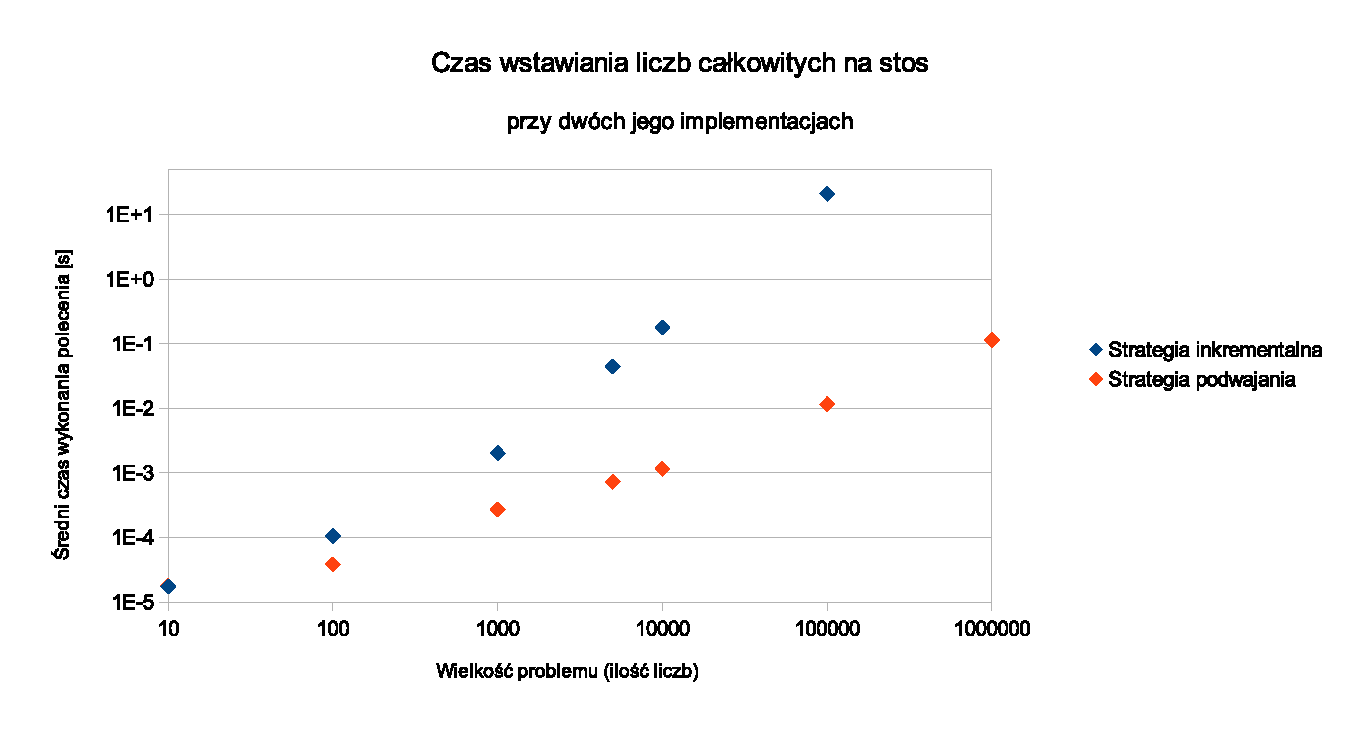
\includegraphics[width=\textwidth]{wykr.eps}
\end{figure}

\section{Wnioski}
\par We wszystkich przypadkach strategia podwajania okazała się szybsza.
Różnica w czasie wykonania wypełnienia stosu stała się jednak znacząca
dla większych rozmiarów problemu.

\par Strategia inkrementacyjna okazała się mieć złożoność obliczeniową 
\(\Theta(n)\), zaś strategia podwajania -- \(\Theta(n^{2})\).

\end{document}
